\documentclass[oneside,final,14pt,a4paper]{extreport}

\usepackage[htt]{hyphenat}
\usepackage{tempora} % Times New Roman alike font  

\usepackage{siunitx}
\usepackage{vmargin}
\setpapersize{A4}
\setmarginsrb{2.5cm}{2cm}{2cm}{2cm}{0pt}{10mm}{0pt}{13mm}

\usepackage{setspace}
\setstretch{1.5}
\usepackage{indentfirst}
\parindent=1.25cm

%%%%% ADDED TO SUPPORT TT BOLD FACES %%%%
\DeclareFontShape{OT1}{cmtt}{bx}{n}{<5><6><7><8><9><10><10.95><12><14.4><17.28><20.74><24.88>cmttb10}{}
\renewcommand{\ttdefault}{pcr}
%%%%% END %%%%%%%%%%%%%%%%%%%%%%%%%%%%%%% 

\usepackage{atbegshi,picture}
\usepackage[T1,T2A]{fontenc}
\usepackage[utf8]{inputenc}

\usepackage[english]{babel}
\usepackage[backend=biber,style=ieee,autocite=inline]{biblatex}
\bibliography{ref.bib}
\DefineBibliographyStrings{english}{%
  bibliography = {References},}
\usepackage{blindtext}

\usepackage{pdfpages}
\newenvironment{bottompar}{\par\vspace*{\fill}}{\clearpage}
\usepackage{amsmath,amsfonts}
\usepackage{url}
\usepackage{amsthm}
\newtheorem{theorem}{Theorem}
\newtheorem{corollary}{Corollary}
\newtheorem{lemma}{Lemma}
\newtheorem{proposition}{Proposition}
\theoremstyle{definition}
\newtheorem{definition}{Definition}
\theoremstyle{remark}
\newtheorem*{remark}{Remark}
\theoremstyle{remark}
\newtheorem*{example}{Example}

\usepackage{float}
\usepackage{graphicx}
\graphicspath{{figs/}} %path to images
\usepackage{array}
\usepackage{multirow,array}
\usepackage{caption}
\usepackage{subcaption}
\usepackage{hyperref}
\hypersetup{colorlinks=true, linkcolor=black, citecolor=black}
\usepackage{paralist}
\usepackage{listings}
\usepackage{zed-csp}
\usepackage{fancyhdr}
\usepackage{csquotes}
\usepackage{color}
% \usepackage{anyfontsize}
% \usepackage{mathptmx}
% \usepackage{t1enc}

\usepackage{chngcntr}
\usepackage{upgreek} 
\usepackage{bm}
\usepackage{hyperref}
\usepackage{booktabs}
\usepackage{multirow}
\usepackage{longtable}
\usepackage[font=singlespacing, labelfont=bf]{caption}
%Hints
\newcommand\pic[1]{(Fig. \ref{#1})} %Ref on figure
\newcommand\tab[1]{(Tab. \ref{#1})} %Ref on table

\setlength{\headheight}{32.0976pt}
\usepackage{enumitem}
\newlist{inlinelist}{enumerate*}{1}
\setlist*[inlinelist,1]{%
  label=(\arabic*),
}

% \setcounter{secnumdepth}{4}
\captionsetup[table]{labelfont={normalfont}, name={TABLE}, labelsep={newline}}
\setlength{\parindent}{2em} 
\DeclareCaptionLabelSeparator{figSep}{.\quad}
\captionsetup[figure]{labelfont={normalfont}, name={Fig.}, labelsep=period, justification=raggedright}
\counterwithin{figure}{chapter}

% \usepackage{titlesec}
% \titleformat{\section}[hang]{\fontsize{20}{24}\selectfont\filcenter}{\Roman{section}}{1em}{}
% \titleformat{\subsection}[hang]{\itshape}{\Alph{subsection}.}{1em}{}[]
% \titleformat{\subsubsection}[runin]{\itshape}{\arabic{subsubsection})}{1em}{}[$:$]
% \titlespacing{\subsubsection}{1em}{1em}{1em}
% \titleformat{\paragraph}[runin]{\itshape}{\alph{paragraph})}{1em}{}[$:$\quad]
% \titlespacing{\paragraph}{2em}{1em}{1em}

\usepackage{placeins} % for \FloatBarrier

\pagestyle{fancyplain}

% remember section title
\renewcommand{\chaptermark}[1]%
	{\markboth{\chaptername~\thechapter~--~#1}{}}

% subsection number and title
\renewcommand{\sectionmark}[1]%
	{\markright{\thesection\ #1}}

\rhead[\fancyplain{}{\bf\leftmark}]%
      {\fancyplain{}{\bf\thepage}}
\lhead[\fancyplain{}{\bf\thepage}]%
      {\fancyplain{}{\bf\rightmark}}
\cfoot{} %bfseries


\newcommand{\dedication}[1]
   {\thispagestyle{empty}
     
   \begin{flushleft}\raggedleft #1\end{flushleft}
}

\begin{document}

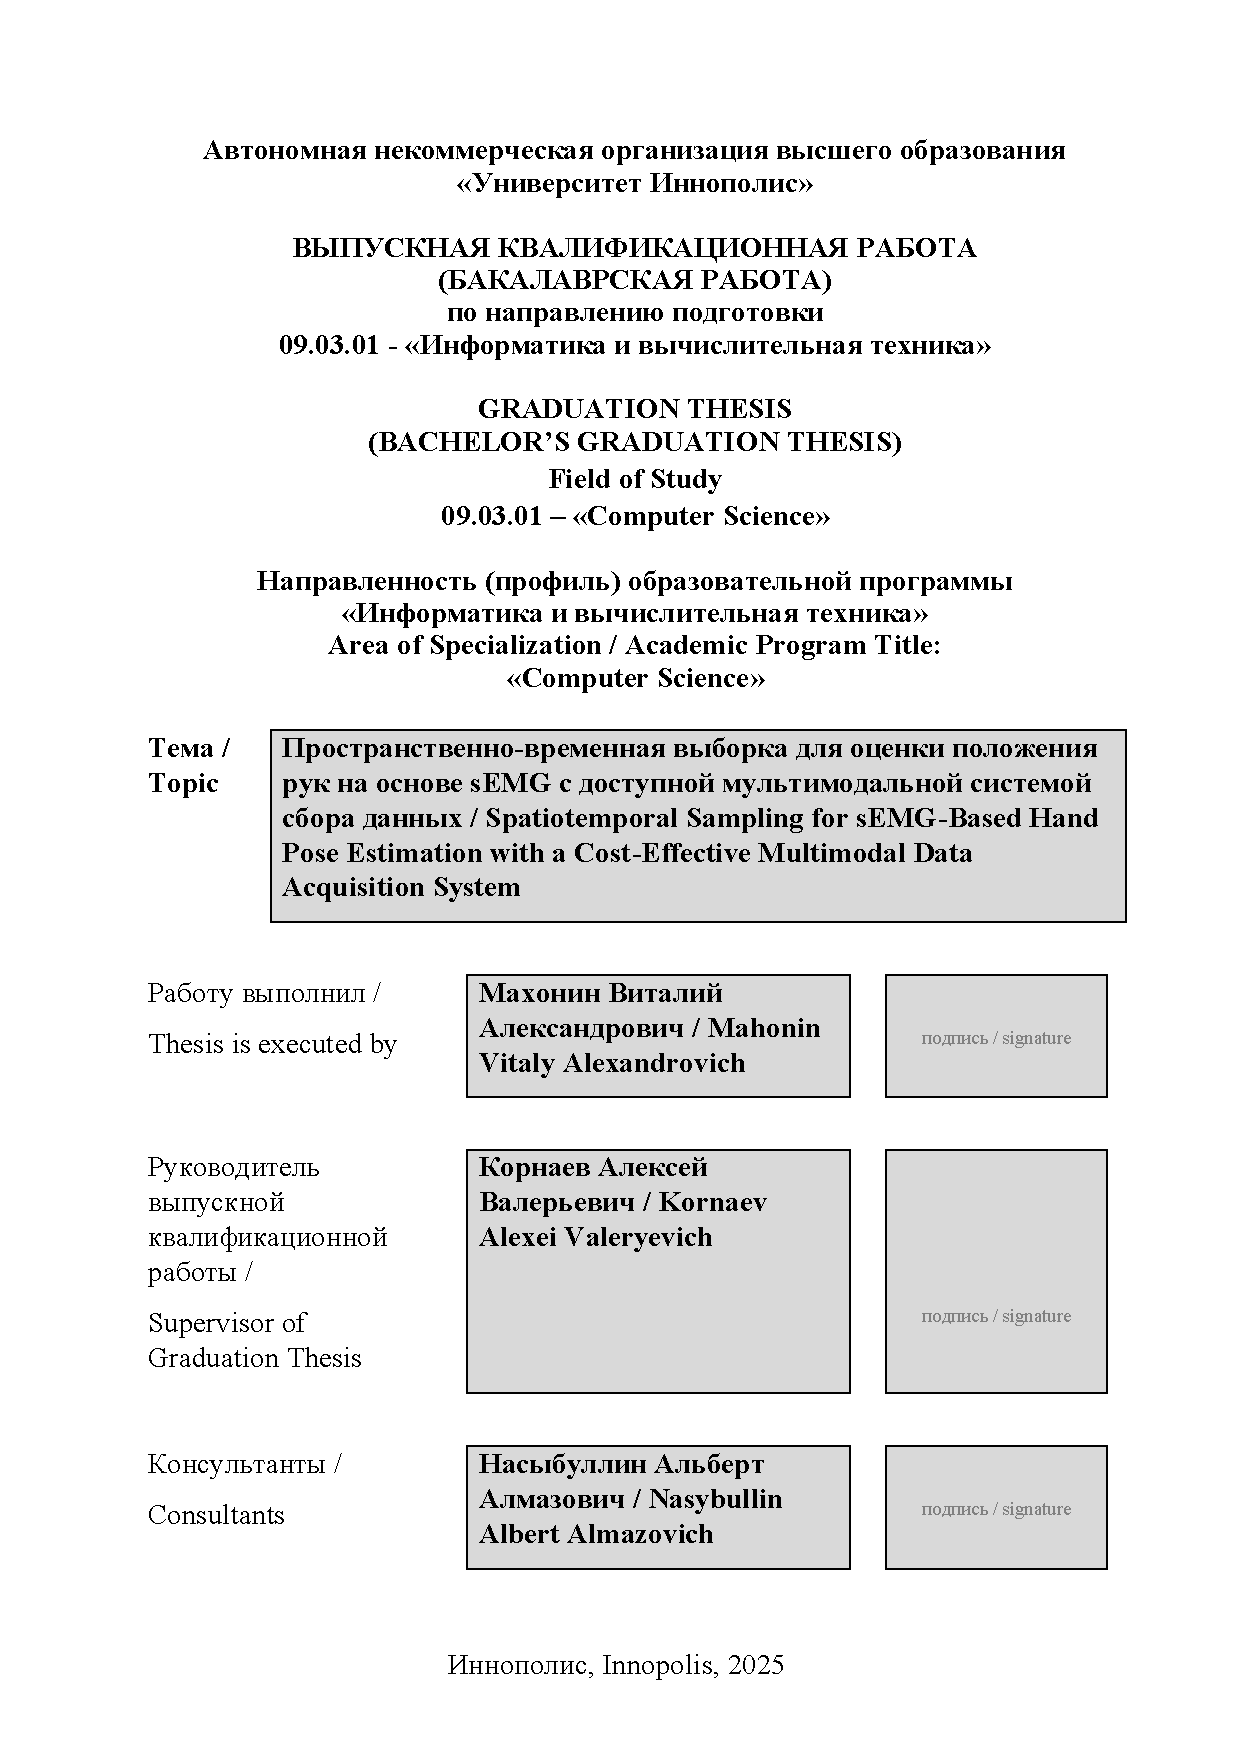
\includepdf[pages=-]{title.pdf}
\tableofcontents
\listoftables
\listoffigures
\newpage


\begin{abstract}
% skip one line to make the abstract start with indent

My abstract starts from here.
\end{abstract}
\setcounter{page}{7}
% set manually the number, from which Chapter 1 starts!
% Why do we put 7 in this case?
% Title page - page 1
% Contents - page 2, page 3
% List of tables - page 4
% List of figures - page 5
% Abstract - page 6
% Chapter 1 - page 7
% In your thesis the counter number can be different, please count carefully and insert the corresponding number.

\chapter{Introduction}
\label{chap:intro}
\chaptermark{Optional running chapter heading}
\section{Spacing \& Type}
\label{sec:section}

This is a section. This is a citation without brackets. and this is one with brackets \cite{A}. Multiple \cite{A,B,C} Here's a reference to a subsection: \ref{sec:subsection}. Citation of an online article \cite{D}. Citation of an online proceeding \cite{F}. The body of the text and abstract must be double-spaced except for footnotes or long quotations. Fonts such as Times Roman, Bookman, New Century Schoolbook, Garamond, Palatine, and Courier are acceptable and commonly found on most computers. The same type must be used throughout the body of the text. The font size must be 10 point or larger and footnotes\footnote{This is a footnote.} must be two sizes smaller than the text\footnote{This is another footnote.} but no smaller than eight points. Chapter, section, or other headings should be of a consistent font and size throughout the ETD, as should labels for illustrations, charts, and figures.

\subsection{Creating a Subsection}
\label{sec:subsection}

\subsubsection{Creating a Subsubsection}
\subsubsection{Creating a Subsubsection}
\subsubsection{Creating a Subsubsection}

\paragraph{This is a heading level below subsubsection}

And this is a quote: 
%
\begin{quote}
\blindtext
\end{quote}

\begin{figure}[hbt]
\centering

\includegraphics[]{figs/images.png}
\caption{One kernel at $x_s$ (\emph{dotted kernel}) or two kernels at
$x_i$ and $x_j$ (\textit{left and right}) lead to the same summed estimate
at $x_s$. This shows a figure consisting of different types of
lines. Elements of the figure described in the caption should be set in
italics, in parentheses, as shown in this sample caption.}
\label{fig:example}
\end{figure}

This is a table:
% currsize is not set in the long table environment, so we need to set it before we set it up.
\makeatletter
\let\@currsize\normalsize
\makeatother

% tabular environments are set to be single-spaced in the  thesis class,  but long tables do not use tabular
% to get around this, set the spacing to single spacing at the start of the long table environment, and set it back to double-spacing at the end of it

\begin{longtable}{c|c|c}
\caption[This is the title I want to appear in the List of Tables]{This Is a Table Example} \label{tab:pfams} \\
\hline
A & B & C \\
\hline
\endfirsthead
\multicolumn{3}{@{}l}{} \\
\hline
A & B & C\\
\hline
\endhead
a1 & b1 & c1 \\
a2 & b2 & c2\\
a3 & b3 & c3\\
a4 & b4 & c4\\
\hline
\end{longtable}

The package ``upgreek'' allows us to use non-italicized lower-case greek letters. See for yourself: $\upbeta$, $\bm\upbeta$, $\beta$, $\bm\beta$. Next is a numbered equation:
\begin{align}
\label{eq:name}
\|\bm{X}\|_{2,1}={\underbrace{\sum_{j=1}^nf_j(\bm{X})}_{\text{convex}}}=\sum_{j=1}^n\|\bm{X}_{.,j}\|_2
\end{align}
The reference to equation (\ref{eq:name}) is clickable. 
\section[Theorems, Corollaries, Lemmas, Proofs, Remarks, Definitions and Examples]{Theorems, Corollaries, Lemmas, Proofs, Remarks, Definitions,and Examples}

\begin{theorem}
\label{thm:onlytheorem}
\blindtext
\end{theorem}

\begin{proof}
I'm a (very short) proof.
\end{proof}

\begin{lemma}
I'm a lemma.
\end{lemma}

\begin{corollary}
I include a reference to Thm. \ref{thm:onlytheorem}.
\end{corollary}

\begin{proposition}
I'm a proposition.
\end{proposition}

\begin{remark}
I'm a remark. 
\end{remark}

\begin{definition}
I'm a definition. I'm a definition. I'm a definition. I'm a definition. I'm a definition. I'm a definition. I'm a definition. I'm a definition. I'm a definition. I'm a definition. I'm a definition. 
\end{definition}

\begin{example}
I'm an example.
\end{example}


\section[Optional table of contents heading]{Section with\\ linebreaks in\\the
name}


\Blindtext[2]





\chapter{Literature Review}
\label{chap:lr}
\chaptermark{Literature Review}

\section{sEMG-Based Hand Pose Estimation}

Surface electromyography (sEMG) is commonly employed to infer hand gestures and joint angles by recording the electrical signals generated in the forearm muscles \cite{oskoei2007myoelectric, simao2019review}. Classic pipelines begin with manually engineered signal descriptors -- like mean absolute value, waveform length, or zero-crossing counts -- and then feed them into classifiers such as Support Vector Machines (SVMs) or Multilayer Perceptrons (MLPs) \cite{oladazimi2012review, liu2007recognition}. Yet these approaches usually struggle to stay reliable when the motions get more complex or the EMG signals vary \cite{parajuli2019real}. On top of that, crafting strong hand-made features usually demands specialized know-how and plenty of expert tweaking, which naturally holds back how well the method transfers to new tasks or users and how easily it can scale \cite{atzori2016deep, oskoei2008support, phinyomark2018feature}.

Recent work has focused on deep learning models, researchers have shifted their attention to deep-learning architectures such as convolutional neural networks (CNNs), recurrent neural networks (RNNs), and temporal convolutional networks (TCNs) \cite{ameri2019regression, briouza2021convolutional, zhang2023lstm}. These networks can pull out time-based patterns straight from raw or lightly processed sEMG. Even though they usually beat the classic feature-engineering pipelines in accuracy, they still stick to dynamic pattern search and are expensive at compute. \cite{lee2022explainable}.

To address this gap, some studies have turned to attention-driven and adaptive networks that can zero in on the most informative parts of the EMG signal \cite{yang2025stcnet, hu2019semg}. Yet, few works introduce generally new novel techniques, especially the ones aiming to reduce compute by leveraging the signal nature itself. Our proposed approach, termed \textit{Spatiotemporal Sampling}, aims to fill this gap by learning a sampling window and spatial activation pattern jointly from the data.

\section{Multimodal sEMG Datasets}

Several public datasets now support training and evaluating sEMG-based models. Among them, the \textbf{NinaPro} series is the go-to choice, pairing synchronized sEMG signals with kinematic-glove readings across many gesture types \cite{zia2018multiday}. Despite its usefulness, NinaPro centers on brief, scripted motions and cross-subject generalization, so it is less ideal for single-user studies that need longer, continuous recording sessions.

The \textbf{EMG2Pose} dataset represents one of the most ambitious publicly released resources for fine-grained pose regression to date \cite{salter2024emg2pose}. It blends high-resolution 3-D motion-capture data with simultaneously recorded sEMG signals obtained from 26 OptiTrack cameras and state-of-the-art Delsys electrodes -- an impressive yet cost-prohibitive arrangement for most academic laboratories. In a similar vein, leading studies on continuous hand tracking routinely acquire sEMG at sampling rates near 2 kHz and with at least 12-bit resolution -- technical choices that safeguard subtle muscle-activation details and the sub-millisecond timing needed for accurate joint-angle estimation \cite{salter2024emg2pose, zanghieri2023semg, lee2022explainable}. Consequently, these hardware specifications have become the de facto yardstick for high-resolution EMG-to-pose research, setting a performance bar that lower-cost systems must now strive to meet.

At the opposite end of the price range, a variety of very low-cost rigs have appeared -- often built around consumer devices such as the Myo armband or custom EMG boards powered by Arduino controllers \cite{nasri2020semg}. Although appealing for their affordability, these setups usually face two major hurdles:
\begin{itemize}
    \item Sampling resolution and rates that fall short of the \(\sim\!12\text{-bit}\), \(2\,\text{kHz}\) baseline;
    \item No reliably synchronized, continuous hand-tracking stream at \(30\,\text{fps}\) or higher \cite{graf2023combining}.
\end{itemize}

\section{3D Hand Tracking with MediaPipe}

MediaPipe is the leading open-source toolkit for 3-D hand tracking in both academic studies and real-world products. Released by Google, it bundles a full graph-based vision pipeline, delivering real-time (30-60 fps) landmark detection, temporal filtering, and gesture classification from nothing more than a standard RGB camera. Because the entire framework is cross-platform -- running on desktop CPUs, mobile phones, and even tiny single-board computers -- it lowers the barrier to entry for labs and start-ups that can`t afford specialised depth sensors.

Unlike closed systems such as the Leap Motion controller or most VR headsets -- which lock users into proprietary hardware, fixed SDKs, and a cramped capture volume of roughly 0.5 - 1 m -- MediaPipe imposes no hard tracking boundary. The same model can follow hands at arm`s length, across a lab bench, or within a wide-angle studio shot, enabling what we call \textit{unbounded spatial scaling}. Its permissive licence also lets researchers tweak the network architecture, integrate domain-specific priors (e.g., EMG synchronisation), and port the solution to custom embedded boards -- fostering rapid experimentation that would be impossible on locked-down commercial stacks. In short, MediaPipe blends affordability, flexibility, and high frame-rate performance, making it an ideal backbone for our cost-efficient, multimodal data-collection system.

Several independent investigations now provide quantitative proof that MediaPipe delivers both high accuracy and robustness across a broad spectrum of experimental conditions. For example, Reimer \textit{et al.} \cite{reimer2023evaluation} ran a room-scale benchmark showing that the framework can keep a stable lock on the hand skeleton at viewing distances of up to 2.75 m -- a range in which the Oculus Quest optical tracker and the Leap Motion controller already begin to show noticeable drop-outs, especially when multiple users move simultaneously in the same capture space.  

When the focus shifts to fine-grained finger-joint reconstruction, Maggioni \textit{et al.} \cite{maggioni2025optimisation} recorded a RMSE of just \(10.9^{\circ}\) joint angle error for MediaPipe -- comfortably below the \(14.7^{\circ}\) reported for Leap Motion in the identical task -- underlining the framework`s superior kinematic fidelity.  

Beyond pure motion capture, Lee \textit{et al.} \cite{lee2022explainable} have already integrated MediaPipe-derived landmarks into deep-learning pipelines for sEMG-based gesture recognition, further reinforcing its value as a dependable, high-quality data source for multimodal research and practical applications.

Taken together, these strengths make MediaPipe an ever more compelling solution for conventional motion-capture systems -- particularly in research or industrial settings that need 3-D hand-pose tracking which scales easily, stays budget-friendly, and still meets strict accuracy requirements.

\section{Deep Learning Models for EMG-to-Pose Estimation}

Early deep-learning efforts showed that both convolutional and recurrent networks can handle \textit{sEMG} signals for hand-gesture recognition. Briouza \textit{et al.} \cite{briouza2021convolutional}, for example, built a compact 1-D CNN that reached high accuracy on the Ninapro DB2 benchmark (49 gestures across 40 participants). A newer study by Zhang \textit{et al.} \cite{zhang2023lstm} introduced an LSTM with a two-stage attention module (LSTM-MSA) that surpassed earlier models on several EMG datasets, boosting F1-score, accuracy, recall, and precision. These findings underline how adding temporal context and learned attention can greatly improve sEMG decoding.

The field is now shifting from classifying discrete gestures to \textit{continuous pose estimation}. In this newer line of work, networks aim to map raw sEMG directly to full hand kinematics, predicting joint angles frame by frame.

\textbf{VEMG2Pose} -- introduced together with the EMG2Pose dataset -- adopts a velocity-first decoding strategy \cite{salter2024emg2pose}. A time-depth separable CNN encoder first grabs features, after which an LSTM predicts angular velocities from the sEMG and integrates them over time into joint angles. This autoregressive loop smooths trajectories and keeps drift in check. Even though the network has only a few million parameters -- roughly on par with other baselines -- it still delivers state-of-the-art results. In EMG2Pose`s toughest split (unseen users and unseen motion stages), it posted the lowest mean fingertip landmark error at \textbf{21.6 \textpm 2.0 mm}, outperforming NeuroPose (24.9 \textpm 1.7 mm) and SensingDynamics (27.2 \textpm 2.0 mm) under the same protocol. Its mean joint-angle error in that scenario was 15.8$^\circ$, versus 17.5$^\circ$ and 18.7$^\circ$ for the competing models. VEMG2Pose also leads in the easier generalization tasks -- evidence that velocity decoding boosts cross-user robustness. The model further benefits from being trained on the massive EMG2Pose collection comprising \textbf{193 subjects and 370 hours} of sEMG-motion data, which likely enhances its ability to cope with varied users and gestures.

\textbf{NeuroPose} takes a different route -- it performs \emph{direct} joint-angle regression with a U-Net-style encoder-decoder built from residual bottleneck blocks \cite{liu2021neuropose}. A convolutional encoder first compresses the multi-channel sEMG signal in both space and time, residual layers refine the features, and a decoder upsamples the representation back to the original rate to output joint angles frame by frame.

The earliest version by Liu \textit{et al.} (2021) -- trained on a modest 8-channel Myo armband with only 12 users -- employed anatomical finger-motion constraints plus transfer learning to adapt to new participants. It reported a median angular error of roughly \textbf{6.24$^\circ$} (90th percentile 18.3$^\circ$) and could run in real time on a smartphone with about 0.1 s latency.

To boost interpretability, newer variants weave in attention mechanisms. For instance, Lee \textit{et al.} \cite{lee2022explainable} inserted a channel-wise attention block that highlights which electrode streams matter most for each predicted finger angle, yielding clear saliency maps that align with known muscle activations.

When NeuroPose was retrained from scratch on the larger 16-channel \textit{EMG2Pose} dataset, it remained competitive. Yet, its errors were still higher than those of VEMG2Pose -- for example, a fingertip landmark error of about \textbf{24.9 mm} in the toughest unseen-user split, roughly 15 \% worse \cite{salter2024emg2pose}.

The encoder-decoder (on the order of a few million parameters) and the built-in temporal-smoothing loss do produce smooth trajectories, but the model appears to generalise less effectively to entirely new users without additional adaptation.

\textbf{SensingDynamics} explores yet another design trade-off, pairing \textit{high-density EMG} acquisition with a deliberately lightweight network architecture -- \cite{simpetru10sensing}.
S\^{i}mpetru \textit{et~al.} (2022) recorded signals from a \textit{320-electrode} forearm array distributed across five patches in 13 participants. Their model uses a custom 3-D convolutional encoder to digest the 320-channel spatio-temporal input, followed by a compact three-layer MLP that simultaneously predicts joint angles, key-point positions, and even grip force. According to their report, the system can \emph{"sense the full dynamics"} of the hand, reaching within-subject fingertip errors as low as \textbf{3 mm} (MAE).

Because the network was tuned specifically for this dense layout, it includes layers such as learnable synthetic-muscle-unit (SMU) activations, 3-D convolutions that span multiple electrode patches, and a parallel low-pass EMG branch to boost noise robustness. Even with these extras, SensingDynamics remains the most parameter-efficient of the three baselines -- only a handful of convolutional blocks plus a small MLP. That compactness, however, comes with a trade-off: on the larger cross-user benchmark it lags behind the other models, posting roughly \textbf{27.2 mm} mean fingertip error in the unseen-user-and-stage split -- versus 24.9 mm for NeuroPose and 21.6 mm for VEMG2Pose. In short, its streamlined architecture excels on its original high-density, per-user data but struggles to capture the fuller signal complexity required for broad generalisation.

All three baseline models were re-examined under a single evaluation pipeline in the EMG2Pose study \cite{salter2024emg2pose}, after being retrained on the project`s full corpus of roughly \(\sim\!80\) million frames from 193 participants. The head-to-head results highlight three main takeaways.  
\textbf{First}, networks that treat temporal dynamics explicitly -- as VEMG2Pose does through its velocity-integration loop -- deliver smoother trajectories and lower errors.  
\textbf{Second}, generalisation hinges on both model capacity and data scale: SensingDynamics, although highly accurate in its original per-user, high-density setting, falls behind on this broader, more varied dataset.  
\textbf{Third}, interpretability add-ons -- for example, the channel-wise attention in newer NeuroPose variants -- are becoming essential for diagnosing and refining EMG-to-pose pipelines.  

Informed by these lessons, the present work introduces an \emph{adaptive spatio-temporal sampling} block that automatically highlights the most informative electrodes and time windows on a per-instance basis, aiming to boost intra-user robustness and enhance overall decoding reliability.

\section{Research Gap and Questions}
\label{sec:gap}

Despite rapid progress, sEMG-based hand-pose tracking still suffers from three
core deficiencies: (i) uncertainty over how much performance can be squeezed
from \emph{low-cost hardware}, (ii) lack of a principled way to \emph{sample
spatiotemporal structure} in the EMG stream, and (iii) dataset practices that
let a network "guess" future motion from kinematic continuity alone.  
The thesis addresses these deficits and frames them as the following research
questions (\textbf{RQ-A}, \textbf{RQ-B}, \textbf{RQ-C}).

\subsection*{Gap 1 — Practical limits of budget hardware}

State-of-the-art datasets rely on \(>\)\$20 k motion-capture volumes and
precision sEMG amplifiers; such equipment is unattainable for many research
groups.  It remains unclear how far a frugal rig can go before sensor noise,
latency, or clock drift erase the gains of better algorithms.

\begin{description}[style=unboxed,leftmargin=0pt]
\item[\textbf{RQ-A}] \emph{How well can an inexpensive, four-webcam optical
      setup and a \$40 Seeeduino-based sEMG board support millimetre-accurate
      hand tracking?}  At what point does hardware noise—not model capacity
      become the performance bottleneck?
\end{description}

\subsection*{Gap 2 — Missing adaptive spatiotemporal sampling}

Most networks still use a fixed window and equal weighting for every electrode,
ignoring electromechanical delay, muscle-specific activation, and temporal
context. This wastes computation and obscures physiological meaning.

\begin{description}[style=unboxed,leftmargin=0pt]
\item[\textbf{RQ-B}] \emph{Can a learnable sampler that chooses \textbf{where}
      (electrode) and \textbf{when} (time slice) to look in the EMG improve
      accuracy, and does the benefit persist once signal quality drops?}
\end{description}

\subsection*{Gap 3 — Dataset bias toward scripted motion}

Short, repetitive gestures dominate public corpora.  A model can overfit by
extrapolating smooth joint trajectories rather than attending to EMG. Long,
unscripted motion is needed to force genuine neuromuscular decoding.

\begin{description}[style=unboxed,leftmargin=0pt]
\item[\textbf{RQ-C}] \emph{Does recording minutes-long, random hand activity
      reduce a model`s ability to "cheat" without EMG, and how should such
      sessions be structured and split to study both intra- and inter-subject
      generalisation?}
\end{description}

\chapter{Methodology}
\label{chap:met}
\chaptermark{Methodology}

This chapter documents all engineering steps taken to build and exploit our
custom multimodal sEMG + hand-pose dataset. All code is MIT-licensed; the data
are provided free of charge with no usage restrictions.

\section{Why a New Dataset?}

\begin{itemize}
  \item \textbf{Hardware parity.} EMG2Pose uses 26 OptiTrack cameras and a
        proprietary CTRL-labs wristband -- out of reach for a \$1 000 budget.
  \item \textbf{Temporal realism.} Public corpora favour <10 s gesture clips;
        we require minutes-long, unscripted motion.
  \item \textbf{Storage efficiency.} Using a custom binary format, we
        reduce EMG2Pose`s session files to $\approx2.5\,\%$ of it's size, with no loss of
        information.
\end{itemize}

(An end-to-end tutorial that reproduces every step in this chapter is included
in the top-level README of
\href{https://github.com/Senopiece/emg_hand_pose_dataset_capture/tree/v1.0}{the
capture repository}\footnote{\url{https://github.com/Senopiece/emg_hand_pose_dataset_capture/tree/v1.0}}.)

\section{Four-Camera Hand-Pose Subsystem}

\subsection{Geometry and Calibration}

Four webcams (1280x800, 60 fps) are mounted around a
\SI{1.2}{\metre}$^{3}$ workspace -- three frontal views aimed at the palm and one
dorsal view.  Accurate multi-view geometry is obtained with a \textit{radon
checkerboard}: an \emph{asymmetric} grid printed on \textbf{both} faces of an
A4 sheet, with extra anchor dots so the two patterns coincide perfectly when
held up to the light.  Thanks to this dual-face design every camera can see a
valid checkerboard in the \emph{same} shot, eliminating the 180° ambiguity of
single-face boards.

\begin{enumerate}[label=\arabic*.]
  \item \textbf{Per-camera intrinsics}\\
        \verb|cv::findChessboardCorners| detects the pattern in live frames
        streaming from each webcam.  Once every camera has logged
        $\ge12$ detections, \verb|cv::calibrateCamera| estimates the intrinsic
        matrix $K$ and distortion coefficients~$D$ individually
        (RMS reprojection error < \SI{0.3}{px}).

  \item \textbf{Pair-wise stereo calibration}\\
        One camera is designated the \emph{pivot}; by default the first index
        found in \texttt{cameras.def.json5}.  For each remaining camera, the
        script runs \verb|cv::stereoCalibrate| against the pivot while
        \emph{fixing} the intrinsics from step 1.  
        This yields a rotation $R$ and translation $T$ that map points from the
        pivot’s frame to the partner camera.

  \item \textbf{Write-out and visual check}\\
        All intrinsic blocks and $R\!T$ pairs are dumped to
        \texttt{cameras.calib.json5}.  An optional preview window shows the
        rectified chessboard overlay on every camera so the operator can
        visually confirm alignment before recording.
\end{enumerate}

\noindent
The current implementation relies on direct \emph{pair-wise} overlaps with the
pivot camera; a note in the code highlights a future upgrade to bundle-adjust
\emph{all} pairs for even tighter global consistency.  Nevertheless, the
stereo-against-pivot approach already provides sub-millimetre triangulation
accuracy at a working distance of \SI{50}{\centi\metre}, adequate for EMG-to-pose
learning.

\subsection{Landmark Triangulation \& Real-Time IK}
MediaPipe Hands detects 21 landmarks per retained frame (32 fps after
alignment). Multi-view triangulation yields 3-D key-points. A hand-crafted,
analytic inverse-kinematics solver enforces bone lengths and joint limits and works in real time.

\section{sEMG Acquisition Hardware}

\subsection{Electrode Montage}
Twelve Ag/AgCl electrodes form four bipolar channels + reference:

\begin{enumerate}[label=\alph*]
  \item \textbf{FDS} - \emph{Flexor Digitorum Superficialis}: the main finger-flexor mass on the palmar-ulnar side; activates when the fingers close.
  \item \textbf{FCR} - \emph{Flexor Carpi Radialis}: wrist flexor on the palmar-radial side; contributes to wrist flexion and radial deviation.
  \item \textbf{EDC} - \emph{Extensor Digitorum Communis}: dorsal-radial finger extensors; drives finger extension and assists in wrist extension.
  \item \textbf{ECU} - \emph{Extensor Carpi Ulnaris}: dorsal-ulnar wrist extensor; extends the wrist and produces ulnar deviation.
\end{enumerate}

\subsection{Electronics}
\begin{itemize}
  \item Six Bioelectronic-Circuit amps connected to Seeeduino Xiao (12-bit ADC).
  \item Sampling: \SI{2048}{Hz} x 4 channels.
  \item Streaming: USB 2.0 CDC, sustained $\approx \SI{2}{\mega\bit\per\second}$.
  \item No analogue or digital filtering at capture; any filtering is delegated
        to downstream models.
\end{itemize}

\section{Dataset Infrastructure}
\begin{itemize}
    \item \textbf{Real-time I/O optimisations}.  
          The capture software is build around a multithreaded
          worker-pool design. Careful use of mutexes and ring buffers resolved
          the synchronisation hazards that arise when high-rate EMG and video
          streams are written concurrently to disk.
    \item \textbf{Compact session format}.  
          Each recording session is stored as a single ZIP archive containing
          \textbf{YAML metadata} plus proprietary binary segments for EMG and
          pose.  Compared with an HDF5 dump of the same content, the archive
          shrinks disk usage by roughly \textbf{40x}. The public EMG2Pose
          corpus was re-encoded into this layout so that all datasets share one
          structure.
\end{itemize}

\subsection{Synchronized Recording}

\begin{itemize}
  \item Cameras run at 60 fps; every second frame is kept 32 fps pose stream.
  \item Exactly 64 EMG samples (\SI{31.3}{ms}) align to each pose frame. The
        logger polls the \emph{latest} camera image at each 64-sample boundary.
  \item Timestamp jitter is negligible; no interpolation is
        applied for alignment.
\end{itemize}

\subsection{Session Format}

\paragraph{Layout}

\begin{verbatim}
session.zip/
  metadata.yml
  recordings/
    1/segments/1 2 …
    2/segments/1 2 …
\end{verbatim}

\paragraph{Segment Binary Layout}

Each \texttt{segments/N} file contains a sequence of tuples:

\[
\bigl[
  [\underbrace{20\! \times\! \text{float32}}_{\text{pose}},
   \underbrace{64\!\times\!4}_{\text{EMG}}\text{ float32}],
  \dots,
  \underbrace{20\! \times\! \text{float32}}_{\text{sigma frame}}
\bigr]
\]

The final 20-value \emph{sigma frame} holds the last pose sample that is not coupled with EMG. That is representing the overall intuition of what each patch of the data time alignment is -- meaning that emg timestamp is always captured between pose frames.

\subsection{Quality Control}

The capture application shows

\begin{enumerate}[label=\alph*]
    \item \textbf{EMG oscilloscope}.  
          Scrolling plots of each channel allow the operator to verify signal amplitude, baseline drift, and electrode contact before and during recording.
    \item \textbf{Session control panel}.  
          A GUI window exposes start/stop buttons and a built-in timer that counts elapsed recording time, reducing annotation errors.
    \item \textbf{Interactive 3-D hand preview}.  
          A interactive (rotate/zoom) viewer renders the triangulated skeleton so occlusions or tracking drop-outs can be spotted immediately.
\end{enumerate}

Immediate feedback helps catch loose electrodes or camera drop-outs.

\subsection{Re-encoding EMG2Pose}
Before training, the public EMG2Pose corpus is converted into this exact ZIP
layout using \href{https://github.com/Senopiece/hand_emg_regression/blob/main/notebooks/convert_dataset.ipynb}{the Jupyter workflow}\footnote{\url{https://github.com/Senopiece/hand_emg_regression/blob/main/notebooks/convert_dataset.ipynb}}. This notebook reads the original HDF5
files, extracts pose + EMG, and writes out ZIP packages with YAML metadata,
ensuring both corpora share an identical structure.

\subsection{Interpolation \& Resampling Strategy}

\paragraph{Pose formats.}
The loader supports two 20-angle representations:

\begin{itemize}
  \item \textbf{UmeTrack}  --  the 20-DOF joint-angle vector used in the original
        EMG2Pose release.  For strict comparability with that work, we keep the
        original \emph{linear} interpolation.
  \item \textbf{AnatomicAngles}  --  our own 20-angle layout, reordered to match
        surface-EMG anatomy.  Here we adopt \textbf{Akima splines}, which give
        smoother, overshoot-free trajectories well suited to biomechanical
        data.
\end{itemize}

\paragraph{Kernel benchmark.}
Five interpolation techniques were timed on a 250$\to$1000-frame up-sample test:

\begin{center}\small
\begin{tabular}{@{}lcc@{}}
\toprule
Scheme            & Time (ms) & Visual verdict \\ \midrule
Linear            & 1.0  & robotic, piecewise-constant velocity \\
\textbf{Akima}    & 6.4  & smooth, no overshoot (chosen) \\
Monotone cubic    & 8.3  & smooth but noticeably slower \\
Cubic spline      & 6.7  & severe overshoot at peaks \\
B-spline          & 9.3  & same overshoot issue, slowest \\ \bottomrule
\end{tabular}
\end{center}

Akima offers the best trade-off between speed and anatomical plausibility.

\paragraph{Loader-time resampling.}
Raw pose is stored exactly as captured at 32 fps.  
When a model requests a different label rate (\{16, 32, 64, 128\} fps),
the dataset class resamples on the fly:

\begin{itemize}
  \item \textbf{UmeTrack} $\to$ linear interpolation,
  \item \textbf{AnatomicAngles} $\to$ Akima interpolation.
\end{itemize}

No interpolation is applied during live capture or camera-EMG alignment;
resampling is purely an offline, loader-side convenience.

\subsection{Handling discontinuities and patch sampling.}
Real-world recordings -- especially those in EMG2Pose -- contain brief drop-outs:
marker occlusions, IK failures, or EMG glitches that break a take into smaller
\emph{segments}.  If we naïvely extracted every possible 2-second patch from a
long train/val window, datasets with many discontinuities would yield fewer
valid clips, biasing model comparison.

To keep evaluations fair across both our \emph{single, continuous} recording
and the \emph{multi-segment} EMG2Pose corpus, we adopt a two-tier sampling
strategy:

\begin{enumerate}[label=\arabic*.]

  \item \textbf{Deliberately long windows.}  
        We first carve out generous, non-overlapping intervals -- 
        e.g.\ \texttt{train\_length} = \SI{20}{min} and
        \texttt{val\_length} = \SI{4}{min}.
        Even if a recording is peppered with short gaps, each interval still
        contains enough usable footage.

  \item \textbf{Fixed patch subset.}  
        From each long interval we enumerate every admissible 2-second patch
        (sliding by one frame).
        We then \emph{randomly select a fixed number} of patches
        (\texttt{train\_patches}, \texttt{val\_patches}) -- the same count for
        every dataset run.  
        This normalises the effective sample size: EMG2Pose and our dataset
        each contribute the identical number of train/val clips, regardless of
        how fragmented the underlying footage is.

  \item \textbf{Per-epoch sub-sampling.}  
        During training, only a percentage
        (\texttt{train\_sample\_ratio}, \texttt{val\_sample\_ratio}) of that
        fixed patch pool is drawn each epoch.  
        The subset is reshuffled every epoch (with a deterministic RNG seed per
        run) to improve stochastic coverage without changing the overall clip
        inventory.

\end{enumerate}

This three-step approach -- long windows, fixed patch subset, per-epoch draw -- means
that:

\begin{itemize}
  \item A dataset with dense discontinuities (EMG2Pose) and one that is
        nearly continuous (ours) still contribute \emph{exactly the same}
        number of training and validation clips, eliminating bias from
        uneven patch counts.
  \item Stochastic diversity is preserved across epochs, helping optimization,
        yet the total pool remains constant, keeping cross-model metrics
        strictly comparable.
\end{itemize}

\subsection{Inter-subject time-budget split.}
Unlike our required goal, even within the same session the EMG2Pose corpus contains many short recordings of discrete stage classes.
To evaluate \emph{inter-subject} generalization we apply the time-budget logic \emph{per recording}, ensuring every stage class contributes
a training slice and a validation slice:

\begin{itemize}
  \item For each recording $r_{i}$ (and thus for each subject), draw  
        a random offset, then cut  
        \texttt{train\_length}s $\;\to\;$ \emph{train window}  
        followed immediately by  
        \texttt{val\_length}s $\;\to\;$ \emph{validation window}.
  \item If a recording is too short for both windows, it is skipped; the global
        budgets are re-balanced across the remaining recordings so the overall
        train/val duration is still met.
\end{itemize}

Because the same seconds-based budgets are enforced for \emph{every} recording,
each subject (stage class) is represented evenly in both splits, satisfying the
inter-subject evaluation goal. Coupled with the "long-window $\to$ fixed-patch
subset $\to$ per-epoch draw strategy, this produces a deterministic,
size-matched pipeline that is fair both \emph{within} EMG2Pose and \emph{between}
EMG2Pose and our single-record dataset.

\section{Learning Architecture}
\label{sec:model}

\subsection{Interface and Autoregressive Tracking}

TODO: image

The network operates on a rolling window of sensory history.  
At every step it receives

\begin{itemize}
  \item a \emph{static snapshot} of the most recent EMG slice
        (tens of milliseconds long, covering multiple muscle bursts), and
  \item a \emph{pose context} consisting of the last several hand poses.
        At sequence start these poses come from ground-truth; after the first
        prediction they are replaced by the model’s own outputs.
\end{itemize}

As soon as a new pose is produced, the context window slides forward by one
frame: the oldest pose is discarded, the freshly predicted pose is appended,
and the next EMG slice is read.  
Because this loop has no internal state other than the sliding window itself,
tracking can continue indefinitely on a live EMG stream.

\subsection{Next Pose Prediction}

TODO: image

\begin{enumerate}[label=\arabic*.]
  \item \textbf{EMG featuriser}.  
        Raw multi-channel EMG is transformed into a dense activation vector.
        Two interchangeable stems are explored.  
        The first is a compact 1-D CNN that captures local temporal patterns;  
        the second is an adaptive \emph{Spatiotemporal-Sampling} (STS) stem that
        learns both where and when to attend within the EMG slice.
  \item \textbf{Context fusion}.  
        The EMG feature vector is concatenated with a flattened summary of the
        pose window-positions, first differences (velocity) and second
        differences (acceleration).  This stacked vector forms a rich snapshot
        of "what the hand is doing now" and "how fast it is changing".
  \item \textbf{Stateless predictor}.
        A lightweight multilayer perceptron maps the fused snapshot to the
        next-frame pose.  Skip connections inject the velocity-acceleration
        sub-vector at multiple depths inside the MLP, ensuring high-frequency
        motion cues are preserved even after several nonlinear transformations.
        These shortcuts stabilise training and help the network respond quickly
        to abrupt muscle activations.
  \item \textbf{Jitter filter}.  
        The raw prediction is combined with the existing pose context by a
        learnable causal filter-effectively a content-aware moving average
        whose weights are trained alongside the rest of the network.  The
        filter damps frame-to-frame noise without introducing noticeable lag.
\end{enumerate}

\subsection{Sequence-level Training Objective}

Training is performed on short sequences (e.g.\ a two-second EMG clip).  
Within each sequence the network steps forward autoregressively, updating its
own context exactly as it would at run time.  Only after the entire rollout is
finished is the composite loss evaluated:

\begin{multline*}
\mathcal{L} =
\underbrace{\mathrm{MSE}_{\text{lm}}(\hat L, L)}_{\text{landmark position}}
+
\underbrace{\mathrm{MSE}_{\text{lm}}(\Delta\hat L, \Delta L)}_{\text{velocity}} \\
+
\underbrace{\mathrm{MSE}_{\text{lm}}(\Delta^{2}\hat L, \Delta^{2}L)}_{\text{acceleration}}
+
\text{L}_{1} + \text{L}_{2} \text{ regularisation}.
\end{multline*}


Here \(L(\cdot)\) denotes 3-D landmarks recovered via a forward-kinematics layer
compatible with the chosen pose format.  The positional term drives spatial
accuracy, while the velocity and acceleration terms penalize jitter and
encourage dynamical consistency.  Parameter regularization keeps the model
compact and reduces over-fitting.  
Optimization uses plain gradient descent; because the network is stateless
apart from its sliding window, no back-propagation through time is required.

\medskip\noindent
In summary, the model marries a learnable EMG encoder, a skip-connected MLP,
and a causal filter into a fully autoregressive hand-pose tracker that can
consume continuous EMG data and produce anatomically plausible joint angles in
real time.

\subsection{Comprehensive hyper-parameter sweep}

To put both featuriser families-CNN and STS-on an equal footing, we perform a
single, unified sweep on the Weights\&Biases (W\&B) platform.  
A Bayesian optimizer proposes configurations; each proposal trains under a
\emph{Hyperband} early-stopping regime (a run must survive 70 iterations to
avoid pruning and is forcibly stopped at 300).  
Mean 3-D landmark error on a fixed validation split is the metric to minimize.

\paragraph{Validation slice (fixed for fairness).}
Regardless of dataset origin, every trial is evaluated on exactly

\begin{itemize}
  \item \textbf{36 seconds of validation footage} drawn from each recording;
  \item a \textbf{2-second prediction horizon} inside that slice;
  \item \textbf{256 validation patches}, of which half are sampled each epoch
        to keep run-time reasonable while leaving the pool unchanged.
\end{itemize}

Locking these numbers removes bias due to clip density or recording length
differences.

\paragraph{Data budget and temporal resolution (swept).}
Conversely, the optimizer may vary how much \emph{training} footage it sees and
at what cadence:

\begin{itemize}
  \item \textbf{Training slice duration}: \SIlist{5;8;12;20;25;30}{min};
  \item \textbf{Prediction horizon during training}: \SIlist{1;2;3;4}{s};
  \item \textbf{Number of training patches}: 7 000 to 200 000;
  \item \textbf{Epoch-sampling ratio}: \SIlist{1;5;10;20}{\%};
  \item \textbf{EMG samples per video frame}: \{16, 32, 64\}  
        (\(\approx\)\SIlist{0.25;0.5;1}{ms} resolution per sample).
\end{itemize}

\paragraph{Loss weighting and regularisation.}
The sweep also searches:

\begin{itemize}
  \item \textbf{Position / velocity / acceleration weights}  
        (\(\kappa_{\text{pos}},\kappa_{\text{vel}},\kappa_{\text{acc}}\))  
        in \{0.1, 1, 10\};
  \item \textbf{L\(_\mathbf{1}\) and L\(_\mathbf{2}\)} regularizers in
        \(\{0,10^{-4},10^{-3},10^{-2},10^{-1},1\}\);
  \item \textbf{Learning-rate} for Adam in \(\{10^{-2},10^{-3},10^{-4}\}\).
\end{itemize}

\paragraph{Pose context and shared MLP widths.}
The size of the sliding pose window and the capacity of the fully connected
stack are treated symmetrically for both stems:

\begin{itemize}
  \item \textbf{Poses in context}: \{3, 4, 8, 12, 20\};  
        velocities and accelerations are derived on-the-fly, so a longer
        window provides richer dynamics at the cost of more parameters.
  \item \textbf{Layer widths} for the synapse MLP, muscle MLP, and predictor
        hidden layer: \{32, 64, 128, 512, 1024\}.  
        Skip connections re-inject \((\text{pose},\dot{\text{pose}},
        \ddot{\text{pose}})\) vectors at each depth regardless of the width
        chosen.
\end{itemize}

\paragraph{STS-specific search axes.}
The adaptive Spatiotemporal-Sampling encoder adds:

\begin{itemize}
  \item \textbf{Number of temporal slices} and \textbf{patterns per slice}:
        \{4, 8, 16, 32, 128, 256\};
  \item \textbf{Slice width / stride}: \SIrange{8}{800}{ms};
  \item \textbf{Max / Std window width / stride}:
        \SIrange{1}{512}{ms}.
\end{itemize}

\paragraph{CNN-specific search axes.}
When the stem is a conventional 1-D CNN, three kernel lengths are swept:

\begin{itemize}
  \item First convolution, second convolution, and output convolution are each
        drawn from  
        \{32, 40, 64, 80, 128, 180, 256, 320, 512, 640, 820, 1024\} samples,
        spanning fine spike detection to half-second envelopes.
\end{itemize}

\paragraph{Dataset mixing and randomisation.}
Every trial points to a pseudo-path  
\texttt{/rand:\,./datasets}.  
At launch, this resolver assembles a fresh session list that blends our own
continuous capture with randomly chosen EMG2Pose sessions.  
Consequently, each hyper-parameter set is vetted on \emph{the full diversity of
subjects, hardware, and motion styles}.  
A fixed random seed ensures reproducibility-identical W\&B IDs rerun the same
training itinerary-while still exposing the optimiser to representative
variance.

In total, millions of theoretical combinations collapse to a practical number
of trials thanks to Hyperband`s pruning: only promising regions of the search
space are explored deeply, and unpromising ones are terminated early, yielding
a compute-efficient yet thorough search.

TODO: best hypers sts vs cnn separate freeze and check on multidataset
TODO: +emg and -emg sweeps for finding the fit without EMG bias
\chapter{Implementation}
\label{chap:impl}
\chaptermark{Implementation}

Thanks to 6 respondents participated in the study, we recorded 6 sessions of random motion 40 minutes each. The dataset is available for free use at \href{https://www.kaggle.com/datasets/nabuki/0-flexemg}{the kaggle}\footnote{\url{https://www.kaggle.com/datasets/nabuki/0-flexemg}}.

For the training we used \emph{A100} and \emph{P100} GPUs provided by \emph{InnoDataHub} and \emph{Kaggle}. Overall hyperparameter sweep was done on $\approx$8k runs -- raw sum of computations add up to about 800 hours of training time (e.g. $\approx$400 hours of compute time for each CNN and STS featurizer).

The same hardware was used for the broader investigation of the best hyperparameters of STS and CNN models and exploring fit without emg, making $\approx$100 more fits on different dataset randomizations with total compute of about 20 more hours.
\chapter{Evaluation and Discussion}
\label{chap:eval}

\ldots
\chapter{Conclusion}
\label{chap:conclusion}
\chaptermark{Conclusion}

\ldots


%% REFERENCES
\printbibliography[heading=bibintoc,title={Bibliography cited}]
\appendix
\chapter{Extra Stuff}
\blindtext

\chapter{Even More Extra Stuff}
\blindtext
\end{document}